\subsection{Worksheet - Lagrange Multipliers \& Atwood Machine}
\begin{p}
Write the constraint equations $f(x,y) = const.$ for $x$ and $y$ for the simple plane pendulum and the Atwood Machine.
\end{p}
\begin{s}
The constraint equation is $f(x, y) = \sqrt{x^2 + y^2} = L$ for the simple pendulum and $f(x, y) = x + y = L$ for the Atwood machine (constrained by length of rope).
\end{s}

\begin{p}
Write down the Hamilton's principle $\delta S(x,y) = 0$ for the two constrained variables $x$ and $y$. If we try to make the action stationary, how would the deviations $\delta x$ and $\delta y$ have to be constrained?
\end{p}
\begin{s}
\begin{align*}
    \delta S + \int\left(\dpd{\LL}{x} - \dod{}{t}\dpd{\LL}{\dot{x}}\right)\delta x dt + \int \left(\dpd{\LL}{y} - \dod{}{}\dpd{\LL}{\dot{y}}\right)\delta y dt = 0
\end{align*}
But, these variations must be constrained as $x$ and $y$ are not independent of one another. We note that $\delta x, \delta y$ obey the constraints.
\end{s}

\begin{p}
For deviations that meet the conditions of the question above, write down the variations of the constraint $\delta f$. Multiply $\delta f$ by an unknown function $\lambda(t)$ and add to $\delta S$.
\end{p}
\begin{s}
\[\delta f = \dpd{f}{x}\delta x + \dpd{f}{y}\delta y = 0\]
As the displacement must leave the constraint unchanged. Hence we may add a $0$ to the total variation of $S$ without changing anything. We therefore write:
\[\delta S = \int \left(\dpd{\LL}{x} + \lambda(t)\dpd{f}{x} - \dod{}{t}\dpd{\LL}{\dot{x}}\right)\delta x \delta t + \int\left(\dpd{\LL}{y} + \lambda(t)\dpd{f}{y} - \dod{}{t}\dpd{\LL}{\dot{y}}\right)\delta y dt = 0\]
\end{s}

\begin{p}
Can $\delta x$ and $\delta y$ be independently varied? The multiplying function of the constraint $\lambda(t)$ is so far undetermined and can be chosen as we wish. What special choice of $\lambda(t)$ makes all of the arguments $\delta x$, $\delta y$, $\delta z$... vanish? How have the Lagrange equations been modified when the dependent variables are constrained?
\end{p}
\begin{s}
Unlike the case with generalized coordinates, the variations are not independent. Consider that we can pick $\lambda (t)$ (Lagrange multiplier) to be whatever we like to make the first integral vanish. However, this then means that the second term must vanish as well, as the sum has to be zero (and if the term is to be zero for all variations, then the integrand must be zero)! In general, if we have a function of (not necessarily generalized coordinates) $\LL(x_k, \dot{x}_k, t)$ with $f_{i}(x_k, t) = 0$ ($m$ holonomic constraints), we can consider the modified Lagrangian:
\[\tilde{L}(x_k, \dot{x}_k, t) = \LL(x_k, \dot{x}_k, t) + \sum_{i=1}^m \lambda_i f_i(x_k, t)\]
And if we require that the variation vanishes $\delta S = 0$, then we get a set of generalized Lagrange equations:
\[\dpd{\LL}{x_k} + \sum_{i=1}^m \lambda_i \dpd{f_i}{x_k} = \dod{}{t}\dpd{\LL}{\dot{x}_k}\]

\end{s}

\begin{center}
    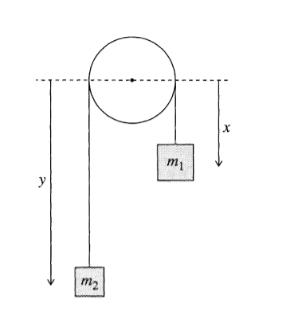
\includegraphics[scale=0.75]{Lecture-8/w8-img1.png}
\end{center}
\begin{p}
What are Lagrange's equations for $x$ and $y$ of the Atwood Machine?
\end{p}
\begin{s}
The Lagrangian is given by:
\[\tilde{\LL} = \LL + \lambda f(x,y) = \frac{m_1}{2}\dot{x}^2 + \frac{m_2}{2}\dot{y}^2 + m_1gx + m_2gy + \lambda(x+y-L)\]
Hence the equations of motions are:
\[m_1\ddot{x} = m_1g + \lambda\]
\[m_2\ddot{y} = m_2g + \lambda\]
Where $\lambda$ is the Lagrange multiplier.
\end{s}

\begin{p}
Using the constraint equation for $x$ and $y$, eliminate the Lagrange multiplier and solveagain for the acceleration of $x$.
\end{p}
\begin{s}
From the constraint equation (taking two time derivatives of it) we obtain that $\ddot{x} = -\ddot{y}$. We therefore have that:
\[\ddot{x} = \frac{(m_1 - m_2)}{(m_1 + m_2)}g\]
\end{s}

\begin{p}
Now solve the equations for the Lagrange multiplier.
\end{p}
\begin{s}
Solving for $\lambda$, we have:
\[\lambda = m_1\ddot{x} - m_1g\]
We note that $m_1\ddot{x}$ is the total force of the system, so
\[m\ddot{x} = -\dpd{U}{x} - F_{T}\]
Where the first term is the conservative (gravitational) force from potential and $F_T$ is the tension/constraint force. Therefore, we have that:
\[\lambda = -F_T\]
And we have found the lagrange multiplier to be the constraint/tension force!
\end{s}

\begin{p}
Show that $\lambda \pd{f}{x}$ s the constraint force on mass $m_1$.
\end{p}
\begin{s}
Here, $\dpd{f}{x} = 1$ so $\lambda\dpd{f}{x} = \lambda = -F_T$ which is the expected result.
\end{s}